\documentclass[12pt]{article}
% LaTeX packages and global styles
% used packages in the template
% import your package here 
\usepackage[utf8]{inputenc}
\usepackage{multicol}
\usepackage{xcolor}
\usepackage{subfigure}
\usepackage{graphicx}
\usepackage{titlesec}
\usepackage[bookmarks,breaklinks,colorlinks=true,allcolors=blue]{hyperref}
\usepackage{listings}
\usepackage{inconsolata}
\usepackage{float}
\usepackage{eso-pic}
\usepackage[framemethod=tikz]{mdframed}
\usepackage[square,numbers]{natbib}
\usepackage{geometry}
\usepackage{amsmath}
\usepackage{parskip}
\usepackage[official]{eurosym}
\usepackage{todonotes}
\usepackage{csquotes}
\usepackage{rotating}
\usepackage{lmodern}
\usepackage{setspace}
\usepackage{tikz} % For flowchart
\usetikzlibrary{shapes.geometric, arrows}
\usepackage{media9} % Required for 3D PDF
\usepackage{listings} % For formatting source code
% style sheet for the thesis
% Chapter and section title format
\titleformat{\section}[block]{\normalfont\huge\bfseries}{\thesection.}{.5em}{\Huge}[{}]
% \titlespacing*{\chapter}{0pt}{-19pt}{25pt}
% \titleformat{\section}[block]{\normalfont\Large\bfseries}{\thesection.}{.5em}{\Large}



% Code listing style
\lstset{
    basicstyle=\ttfamily\small,
    breaklines=true,
    frame=single,
    numbers=left,
    numberstyle=\tiny,
    stepnumber=1,
    numbersep=5pt,
    showstringspaces=false,
    keywordstyle=\color{blue},
    commentstyle=\color{green},
    stringstyle=\color{red},
    backgroundcolor=\color{lightgray!20},
    rulecolor=\color{black},
    captionpos=b
}

% Margins
\geometry{
    a4paper,
    margin=2.75cm
}

% Index depth limit
\setcounter{tocdepth}{2}

% Paragraph Indentation
\setlength{\parindent}{1cm}

\renewcommand{\lstlistingname}{Code extraction}
\renewcommand*{\lstlistlistingname}{Code Excerpts Index}

\definecolor{US_red}{cmyk}{0, 1, 0.65, 0.34}
\definecolor{US_yellow}{cmyk}{0, 0.3, 0.94, 0}

\mdfdefinestyle{US_style}{backgroundcolor=US_yellow!20, font=\bfseries, hidealllines=true}

% Beginning of the document
\begin{document}
    % Title page and unnumbered sections
    \begin{center}
\vspace*{1cm}

\begin{figure}
  \raggedleft
  \begin{minipage}{4cm}
  
\includegraphics[width=4cm]{images/logo1.png}
  \end{minipage}
\end{figure}

\vspace*{2cm}

\vspace*{0.1in}
%yellow version
\AddToShipoutPictureBG*{\AtPageLowerLeft{% 
  \color{lightgray}\rule{.26 \paperwidth}{\paperheight} }
   \:
   \:
   \;
   \;
   \:
  \begin{turn}{90} 
   \fontsize{90}{80}\selectfont \textbf{ \color{white} Report}
  \end{turn}
  
  }

\begin{spacing}{1.7}

\begin{tabular}{p{4cm} ll}

& \textbf{\large Factory Alcohol Detection System}\\ % Here the title of your work 
& \\
& \large Instrumentation Systems (EEE428) \\
& \\
& \large Student: Bayanda Dlamini (202102108)\\
\end{tabular}

\end{spacing}

\end{center}

\thispagestyle{empty} % Prevents page number from being included on the cover
\clearpage\setcounter{page}{1} % Start including page numbers from here
\pagenumbering{roman} % in roman numerals
    %\section*{Abstract}
Workplace safety is a critical concern in industrial environments, particularly in compliance with the Occupational Safety and Health Act, 2001 (No. 9 of 2001) of Eswatini, which mandates safe working conditions for employees. This report presents the design of a Factory Alcohol Detection System to prevent intoxicated employees from entering the workplace. By integrating alcohol detection technology with controlled access, the system ensures compliance with legal standards, reduces workplace hazards, and promotes a safer, more productive environment. The system also logs incidents, aligning with the Act's requirements for hazard monitoring and reporting.

\vspace{.5cm}

\textbf{Keywords:} Alcohol Detection, Workplace Safety, Access Control, Occupational Safety and Health Act
\newpage
    
    % Index of the document and figures
    \begingroup
        \hypersetup{linkcolor=black}
        \tableofcontents
        \listoffigures
    \endgroup
    
    % Change page number style to normal
    \clearpage\pagenumbering{arabic}
    
    % Sections and chapters
    \section{Introduction}
\label{chap:introduction}
Workplace safety is a critical concern in industrial environments, particularly in compliance with the Occupational Safety and Health Act, 2001 (No. 9 of 2001) of Eswatini, which mandates safe working conditions for employees. This report presents the design of a Factory Alcohol Detection System to prevent intoxicated employees from entering the workplace. By integrating alcohol detection technology with controlled access, the system ensures compliance with legal standards, reduces workplace hazards, and promotes a safer, more productive environment. The system also logs incidents, aligning with the Act's requirements for hazard monitoring and reporting.

    % System Overview
    \section{System Overview}
    \label{sec:system_overview}
    The Factory Alcohol Detection System prevents intoxicated employees from entering the workplace. It integrates alcohol detection with access control. The system operates as follows:
    \begin{enumerate}
        \item Employee enters the mantrap.
        \item Identity is verified using fingerprint.
        \item Alcohol sensor analyzes breath sample.
        \item If alcohol level is within limits, exit door opens.
        \item If above limit, alarm triggers, and incident is logged.
        \item Prior records are checked for suspension or dismissal if the limit is exceeded.
    \end{enumerate}

    % Study of the Plant
    \section{Study of the Plant (Factory Entrance and Access Control)}
    \label{sec:plant_study}
    \subsection{Purpose}
    The system regulates employee access, ensuring a safe and secure working environment by preventing intoxicated employees from entering.

    \subsection{Inputs and Outputs}
    \begin{itemize}
        \item Inputs:
        \begin{itemize}
            \item Breath alcohol concentration (BrAC).
            \item Employee identification data (fingerprint).
        \end{itemize}
        \item Outputs:
        \begin{itemize}
            \item Gate access control (open/close signals).
            \item Alarm activation (visual and auditory signals).
            \item Incident logs (employee ID, timestamp, alcohol level).
        \end{itemize}
    \end{itemize}

    \begin{figure}[H]
        \centering
        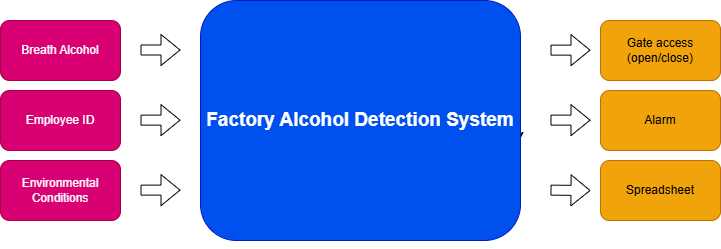
\includegraphics[width=0.8\textwidth]{images/flowChart.png}
        \caption{Block Diagram of Inputs and Outputs}
    \end{figure}

    \subsection{Challenges}
    \begin{itemize}
        \item High employee traffic during shift changes.
        \item Environmental factors (e.g., dust, humidity) affecting sensor performance.
        \item False positives due to ambient alcohol (e.g., cleaning agents).
    \end{itemize}

    % Subsystem Decomposition
    \section{Subsystem Decomposition}
    \label{sec:subsystem_decomposition}
    The system is divided into mechanical, electrical/electronic, and software subsystems.

    \subsection{Mechanical Subsystem}
    \begin{itemize}
        \item Mantrap Structure: Secure enclosure with entry and exit gates.
        \item Gate Mechanism: Electrically controlled doors.
    \end{itemize}

    \subsection{Electrical/Electronic Subsystem}
    \begin{itemize}
        \item Alcohol Sensor: Detects BrAC.
        \item Fingerprint Reader: Verifies identity.
        \item Microcontroller: Processes data and controls actuators.
        \item Actuators: Operate gates and alarms.
    \end{itemize}

    \subsection{Software Subsystem}
    \begin{itemize}
        \item Data Acquisition: Collects sensor data.
        \item Decision-Making Logic: Determines access based on alcohol levels.
        \item Logging and Reporting: Records incidents and generates reports.
    \end{itemize}

    % Operating Requirements
    \section{Operating Requirements (Performance Specifications)}
    \label{sec:operating_requirements}
    \begin{itemize}
        \item Alcohol Detection:
        \begin{itemize}
            \item Detection Range: 0.00\% - 0.20\% BrAC.
            \item Accuracy: $\pm 0.01\%$ BrAC.
            \item Response Time: $\leq 3$ seconds.
        \end{itemize}
        \item Access Control:
        \begin{itemize}
            \item Gate Operation: $\leq 2$ seconds.
        \end{itemize}
        \item Data Logging:
        \begin{itemize}
            \item Storage Capacity: 10,000 records.
        \end{itemize}
        \item Power Requirements:
        \begin{itemize}
            \item Voltage: 24V DC.
            \item Power Consumption: $\leq 50$W.
        \end{itemize}
    \end{itemize}

    % Constraints
    \section{Constraints}
    \label{sec:constraints}
    \begin{itemize}
        \item Size and Weight: Must fit within factory entrance footprint.
        \item Environmental Conditions: Operate in $0^\circ$C to $40^\circ$C and 10\% - 90\% humidity.
        \item Power Requirements: 24V DC, $\leq 50$W.
        \item Security: Tamper-proof data storage and secure communication.
        \item Maintenance: Sensor calibration every 6 months.
        \item Compliance: Occupational Safety and Health Act, 2001 (No. 9 of 2001) of Eswatini.
        \item Compliance: Factory standards
    \end{itemize}

    % Component Selection
    \section{Component Selection}
    \label{sec:component_selection}
    \begin{itemize}
        \item Alcohol Sensor: MQ-3 gas sensor (0.00\% - 0.20\% BAC).
        \item Fingerprint Reader: FPM10A module.
        \item Gate Mechanism: 24V DC electric door locks ($\leq 2$ seconds).
        \item Alarm System: 85 dB buzzer and LED indicators.
        \item Microcontroller: Arduino Uno R3.
        \item Power Supply: 24V DC with overcurrent/overvoltage protection.
        \item Data Storage: SD card module (10,000 records).
    \end{itemize}

    % System Architecture
    \section{System Architecture}
    \label{sec:system_architecture}
    \begin{itemize}
        \item Mechanical Subsystem: Mantrap structure and gates.
        \item Electrical/Electronic Subsystem: Sensors, actuators, and control unit.
        \item Software Subsystem: Data acquisition, decision-making, and logging.
    \end{itemize}

% Flowchart Styles
\tikzstyle{startstop} = [rectangle, rounded corners, minimum width=3cm, minimum height=1cm, text centered, draw=black, fill=red!30]
\tikzstyle{process} = [rectangle, minimum width=3cm, minimum height=1cm, text centered, draw=black, fill=blue!20]
\tikzstyle{decision} = [diamond, minimum width=3cm, minimum height=1cm, text centered, draw=black, fill=yellow!30]
\tikzstyle{arrow} = [thick,->,>=stealth]

% Flowchart
\begin{figure}[H]
    \centering
    \begin{tikzpicture}[node distance=2cm]
        \node (start) [startstop] {Start};
        \node (idCheck) [process, below of=start] {Employee scans ID};
        \node (baseline) [process, below of=idCheck] {Read baseline alcohol level};
        \node (test) [process, below of=baseline] {Employee provides breath sample};
        \node (analyze) [process, below of=test] {Analyze alcohol level};
        \node (decision) [decision, below of=analyze] {Above limit?};
        \node (suspendCheck) [decision, right of=decision, xshift=4cm] {Prior offense?};
        \node (suspend) [startstop, below of=suspendCheck, yshift=-2cm] {Suspend Employee, Log Incident};
        \node (deny) [startstop, above of=suspendCheck, yshift=2cm] {Access Denied, Log Incident};
        \node (allow) [startstop, below of=decision, yshift=-2cm] {Grant Access};
        
        \draw [arrow] (start) -- (idCheck);
        \draw [arrow] (idCheck) -- (baseline);
        \draw [arrow] (baseline) -- (test);
        \draw [arrow] (test) -- (analyze);
        \draw [arrow] (analyze) -- (decision);
        \draw [arrow] (decision.east) -- (suspendCheck.west) node[midway, above] {Yes};
        \draw [arrow] (suspendCheck.north) -- (deny.south) node[midway, right] {No Prior Offense};
        \draw [arrow] (suspendCheck.south) -- (suspend.north) node[midway, right] {Prior Offense};
        \draw [arrow] (decision.south) -- (allow.north) node[midway, right] {No};
    \end{tikzpicture}
    \caption{Flowchart of Alcohol Detection System}
\end{figure}

    % Implementation Plan
%    \section{Implementation Plan}
%    \label{sec:implementation_plan}
%    \begin{itemize}
%        \item Phase 1: Prototype Development (Arduino Uno, MQ-3 sensor).
%        \item Phase 2: Field Testing (real-world installation).
%        \item Phase 3: Full-Scale Deployment (industrial-grade PLC).
%        \item Phase 4: Monitoring and Optimization (continuous improvement).
%    \end{itemize}

    % Conclusion
    \section{Conclusion}
    \label{sec:conclusion}
    The Factory Alcohol Detection System enhances workplace safety by preventing intoxicated employees from entering. It integrates alcohol detection with access control, ensuring compliance with legal standards. Future work will focus on scalability and additional safety features.

    % Appendix
    \appendix
    % Appendix
\section{Schematics and Electrical Drawings}
\label{app:schematics}

This section includes the electrical schematics and wiring diagrams for the Factory Alcohol Detection System.

\subsection{Circuit Diagram}
The circuit diagram for the system is shown in Figure~\ref{fig:circuit_diagram}. It includes the connections for the following components:
\begin{itemize}
    \item Arduino Uno R3 microcontroller.
    \item MQ-3 alcohol sensor.
    \item FPM10A fingerprint reader.
    \item 24V DC electric door locks.
    \item 85 dB buzzer and LED indicators.
    \item SD card module for data logging.
\end{itemize}

\begin{figure}[H]
    \centering
    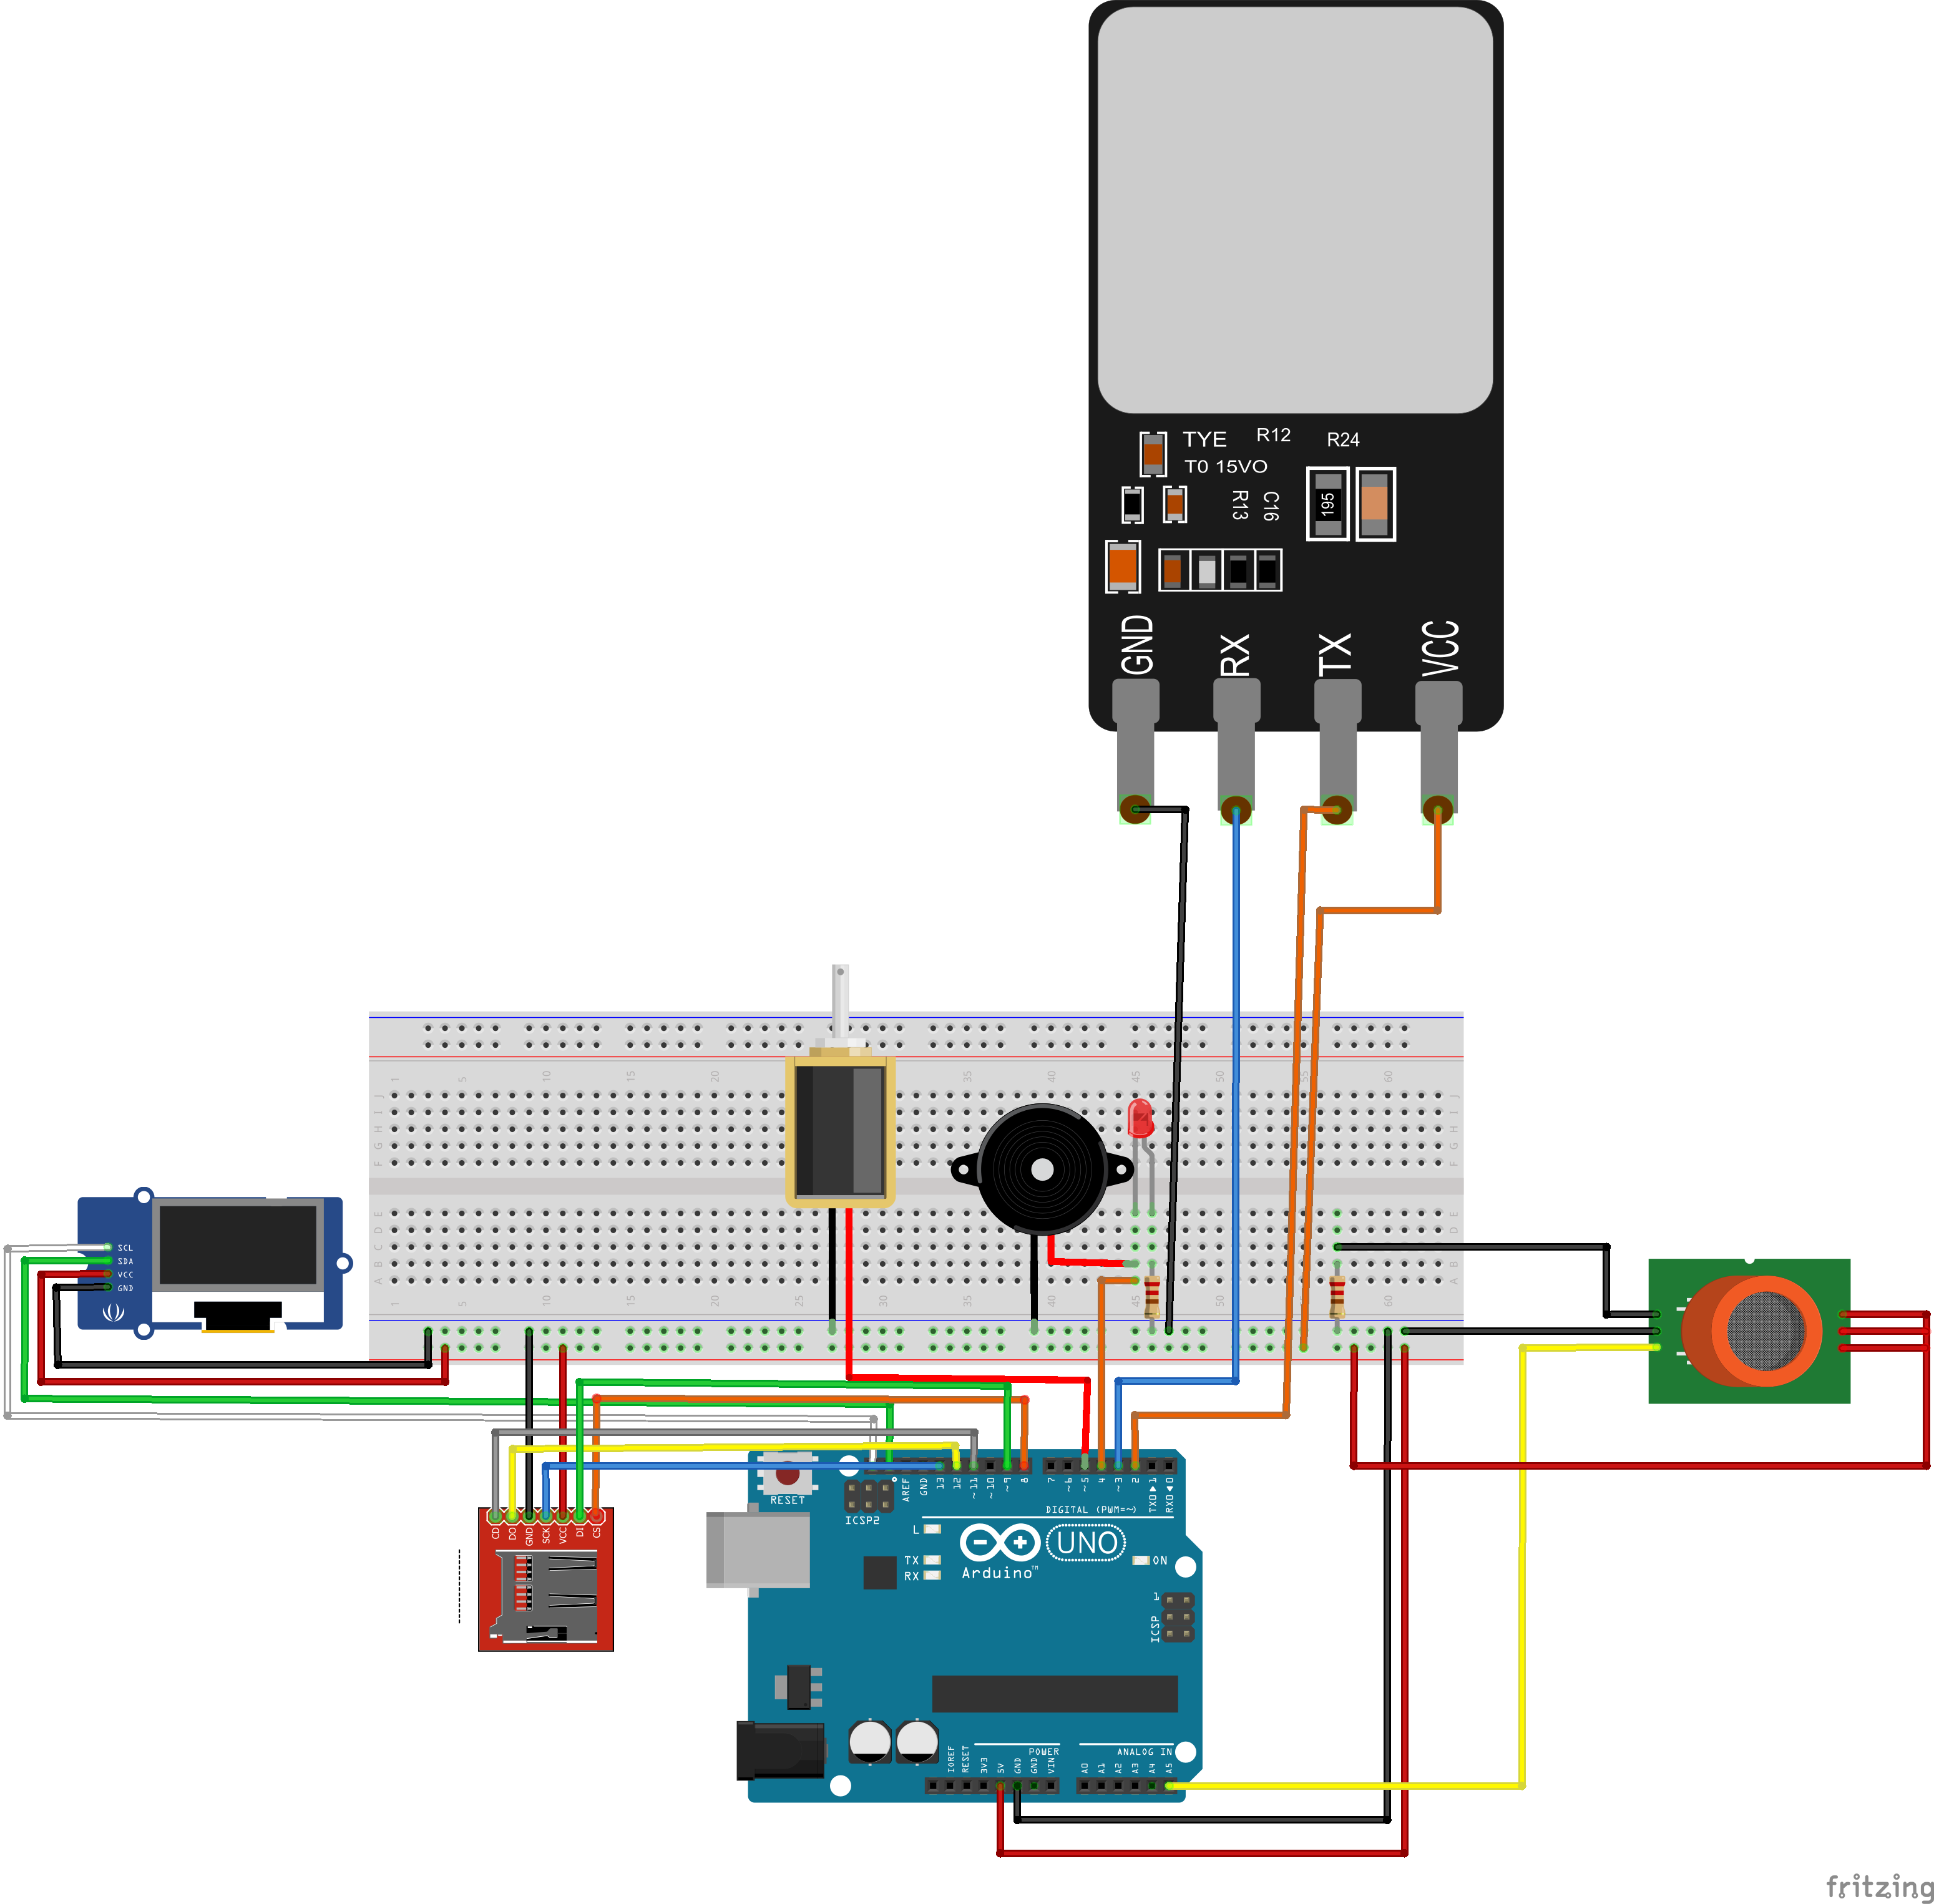
\includegraphics[width=0.8\textwidth]{images/circuit_diagram.png}
    \caption{Circuit Diagram of the Alcohol Detection System}
    \label{fig:circuit_diagram}
\end{figure}
\begin{figure}[H]
    \centering
    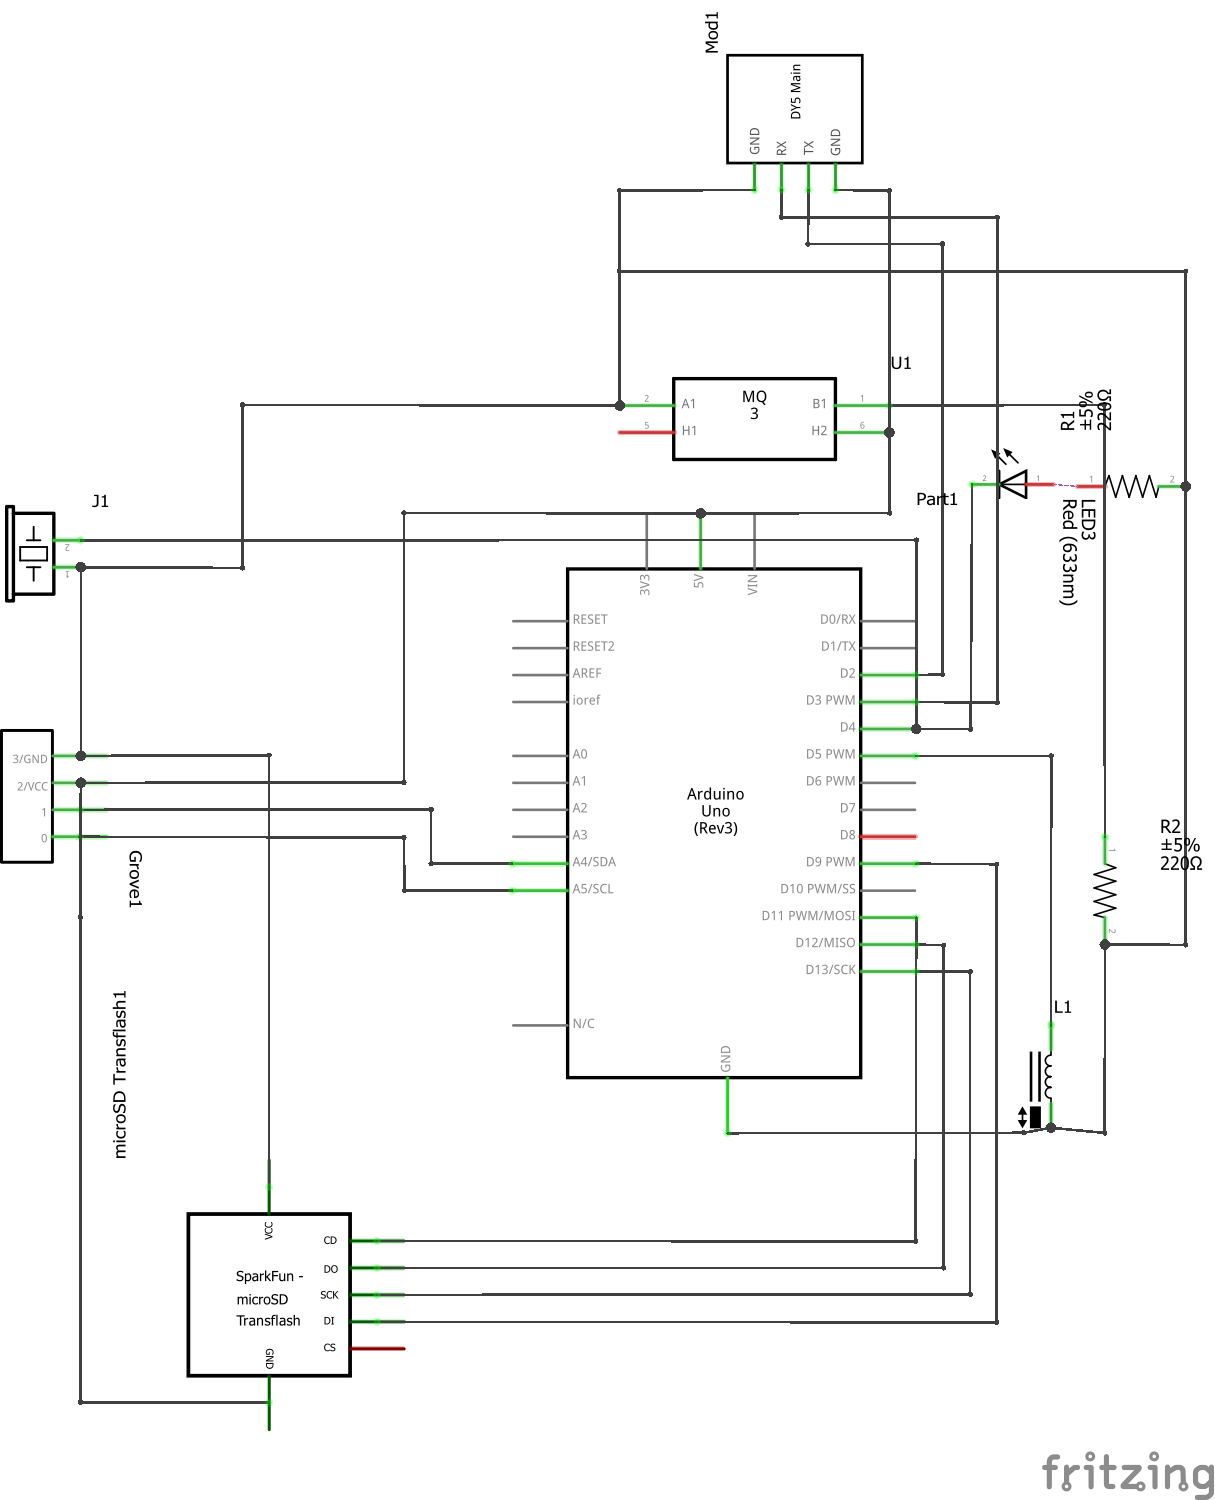
\includegraphics[width=0.8\textwidth]{images/schematic.png}
    \caption{Schematic Diagram of the Alcohol Detection System}
    \label{fig:circuit_diagram}
\end{figure}

\subsection{Power Supply Design}
The power supply circuit provides 24V DC to the system. It includes:
\begin{itemize}
    \item A voltage regulator to ensure stable power delivery.
    \item Overcurrent and overvoltage protection circuits.
\end{itemize}

\section{Mechanical Drawings}
\label{app:mechanical_drawings}

This section includes the image for the mantrap structure and breathalyzer.

% Insert the 3D model
\includemedia[
    width=0.8\textwidth,
    height=0.6\textwidth,
    activate=pageopen,
    3Dmenu,
]{}{images/assembly.u3d}

\subsection{Mantrap Structure}
The mantrap structure is designed to ensure controlled entry and exit of employees. Key features include:
\begin{itemize}
    \item Secure enclosure with entry and exit gates.
    \item Testing chamber for breath sample collection.
\end{itemize}

\begin{figure}[H]
    \centering
    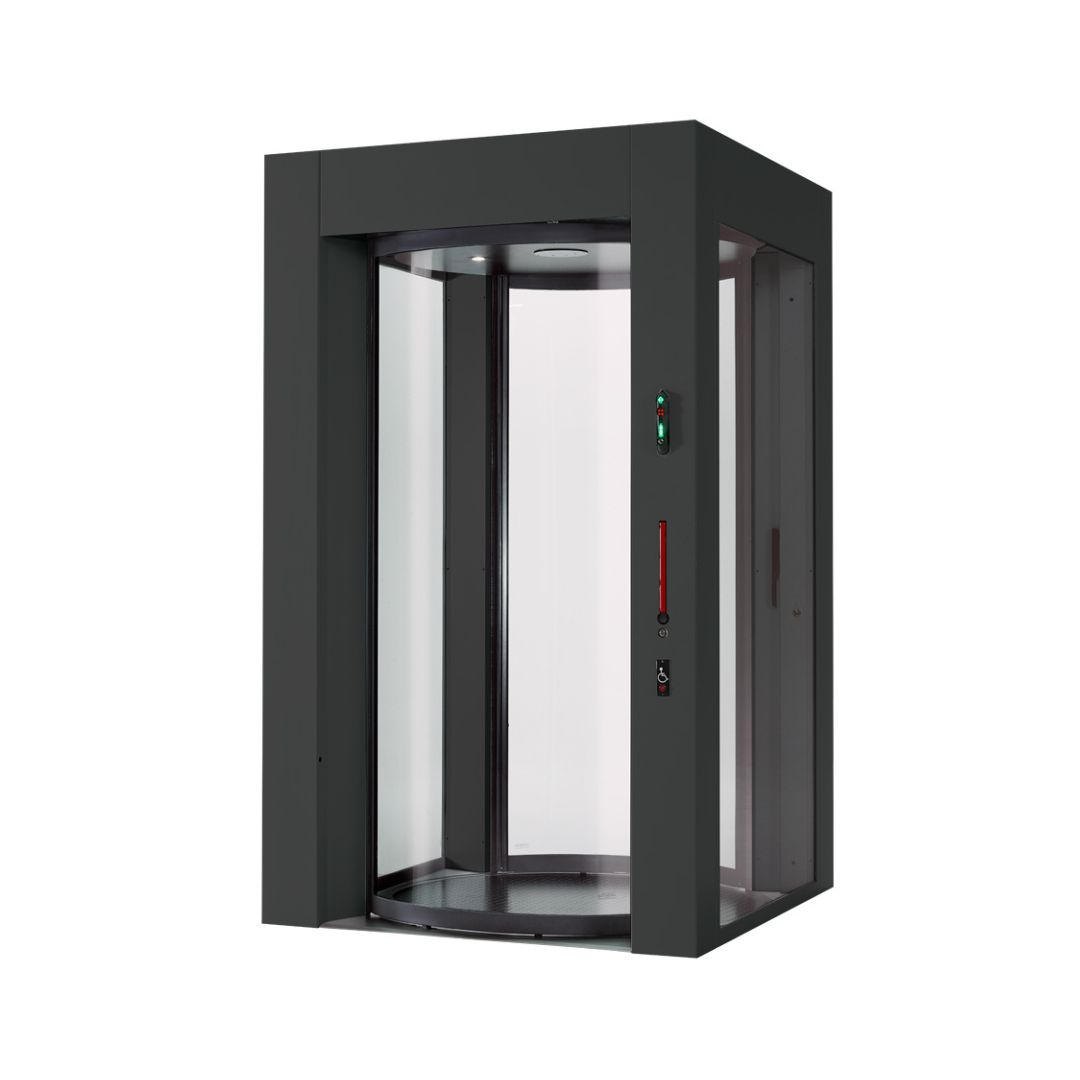
\includegraphics[width=0.8\textwidth]{images/mantrap_drawing.png}
    \caption{Picture of the Mantrap Structure}
    \label{fig:mantrap_drawing}
\end{figure}

\subsection{Gate Mechanism}
The gate mechanism is powered by 24V DC electric door locks. It includes:
\begin{itemize}
    \item Electrically controlled doors with a response time of $\leq 2$ seconds.
    \item Safety sensors to prevent accidental closure.
\end{itemize}

\section{Source Code}
\label{app:source_code}

This section provides the source code for the Factory Alcohol Detection System. The code is written for the Arduino Uno R3 microcontroller.

\subsection{Main Program}
The main program handles data acquisition, decision-making, and logging. Key functionalities include:
\begin{itemize}
    \item Reading data from the MQ-3 alcohol sensor.
    \item Verifying employee identity using the FPM10A fingerprint reader.
    \item Controlling the gate mechanism and alarm system.
    \item Logging incidents to the SD card.
\end{itemize}

\begin{lstlisting}[language=C++, caption={Main Program for Alcohol Detection System}]
#include <SoftwareSerial.h>
#include <SD.h>
#include <FPM.h>

// Pin definitions
const int alcoholSensorPin = A0;
const int gateLockPin = 9;
const int buzzerPin = 10;
const int ledPin = 11;

// Variables
float alcoholLevel;
bool accessGranted = false;

void setup() {
    // Initialize components
    pinMode(alcoholSensorPin, INPUT);
    pinMode(gateLockPin, OUTPUT);
    pinMode(buzzerPin, OUTPUT);
    pinMode(ledPin, OUTPUT);
    Serial.begin(9600);

    // Initialize SD card
    if (!SD.begin(4)) {
        Serial.println("SD card initialization failed!");
        return;
    }
}

void loop() {
    // Read alcohol level
    alcoholLevel = analogRead(alcoholSensorPin) * (5.0 / 1023.0);

    // Check alcohol level
    if (alcoholLevel <= 0.02) {
        accessGranted = true;
        digitalWrite(gateLockPin, HIGH); // Open gate
        digitalWrite(buzzerPin, LOW);    // Turn off alarm
        digitalWrite(ledPin, LOW);       // Turn off LED
    } else {
        accessGranted = false;
        digitalWrite(gateLockPin, LOW);  // Close gate
        digitalWrite(buzzerPin, HIGH);   // Turn on alarm
        digitalWrite(ledPin, HIGH);      // Turn on LED
    }

    // Log incident
    logIncident(alcoholLevel, accessGranted);
    delay(1000);
}

void logIncident(float alcoholLevel, bool accessGranted) {
    File dataFile = SD.open("log.txt", FILE_WRITE);
    if (dataFile) {
        dataFile.print("Alcohol Level: ");
        dataFile.print(alcoholLevel);
        dataFile.print(", Access Granted: ");
        dataFile.println(accessGranted ? "Yes" : "No");
        dataFile.close();
    } else {
        Serial.println("Error opening log file!");
    }
}
\end{lstlisting}

\subsection{Libraries Used}
The following libraries are used in the program:
\begin{itemize}
    \item \texttt{SoftwareSerial.h}: For serial communication with the fingerprint reader.
    \item \texttt{SD.h}: For interfacing with the SD card module.
    \item \texttt{FPM.h}: For interfacing with the FPM10A fingerprint reader.
\end{itemize}

    % Bibliography 
    \bibliographystyle{plainnat}
    \bibliography{bibliography.bib}

% End of the document
\end{document}